\subsection{Rotina de Controle}
\label{subsec:rotina_controle}
Para garantir que não ocorra interrupções o controle é executado sozinho no núcleo secundário (APP CPU) do ESP32. A rotina opera em \emph{Loop} infinito com uma taxa de atualização de $5ms$.\\

Primeiramente a rotina verifica (para cada motor) se tem novas leituras de velocidades, providas pelas interrupções dos sensores, caso tenha, atualiza-se esses valores e prossegue-se para a etapa seguinte. Caso contrário verifica-se a quanto tempo esses valores não são atualizados, caso esse tempo seja superior a um limiar pré-definido (no trabalho usou esse limiar igual a 500ms) considera-se que o motor-roda em questão está parado ($\hat{\omega} = 0$) e avança para a etapa seguinte.\\

Com a informação da velocidade atualizada (ou mantida, caso não houve nova leitura), lê-se as referências para os motores direito e esquerdo. Essas referências inicialmente são valores no intervalo [$-1$, $1$], pois indicam a porcentagem da velocidade que deve ser o \emph{set point} do controlador. \\
% Em seguida calcula-se as referências em rad/s multiplicando-as pela velocidade máxima ($\omega_{max}$) do robô (obtida na etapa de calibração).\\

A etapa seguinte é realizar os cálculos de controle, porém antes disso é necessário passar a referência para $rad/s$, faz-se isso multiplicando as referências relativas (provenientes da comunicação) pela velocidade máxima do robô ($\omega_{max}$), obtida na etapa de calibração. Para então Computar-se separadamente a contribuição do controlador \emph{Feedforward} (conforme \ref{eq:feedforward}) e o proporcional (conforme \ref{eq:proporcional}) para ao final soma-los e ter-se o sinal de controle (PWM/$u(t) \in [-1,1]$). Após o sinal de controle passar por um saturador (para garantir que esteja no intervalo admissível) o sinal PWM para ambos os motores é enviado para o \emph{Driver motor} que tratará de excitar as entradas dos motores com as correspondentes tensões. A Figura \ref{fig:diagrama_de_controle_simplificado} apresenta uma visão geral simplificada do sistema de controle . E a Figura \ref{fig:diagrama_sistema_de_controle_feedforward_backward} ilustra o ciclo de controle \emph{Feedforward} + \emph{Backward}.

\begin{equation}
    u_{ff} = \omega_{ref}\alpha + D
    \label{eq:feedforward}
\end{equation}

\begin{equation}
    u_{p} = (\omega_{ref} - \hat{\omega})K_p
    \label{eq:proporcional}
\end{equation}

\begin{figure}[H]
    \centering
    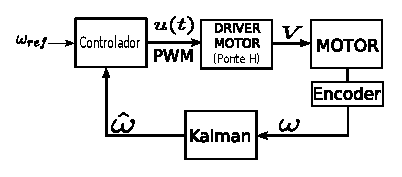
\includegraphics[width=0.5\textwidth]{figuras/ilustracoes/sistema_de_controle_embarcado.eps}
    \caption{Diagrama simplificado do ciclo de controle.}
    \label{fig:diagrama_de_controle_simplificado}
    \fonte{Própria.}
\end{figure}

\begin{figure}[H]
    \centering
    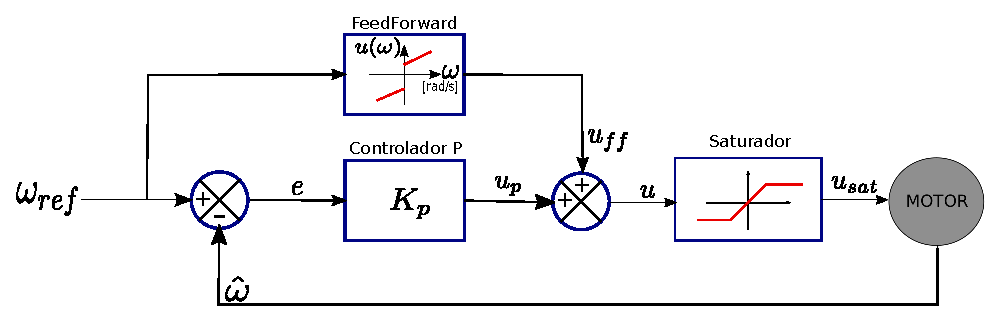
\includegraphics[width=\textwidth]{figuras/ilustracoes/sistema_de_controle_completo.eps}
    \caption{Diagrama de um sistema de controle \textit{Feedforward} + \textit{Backward}}
    \label{fig:diagrama_sistema_de_controle_feedforward_backward}
    \fonte{Própria.}
\end{figure}